\documentclass[tikz,border=5mm]{standalone}
\makeatletter
\newcommand{\Letter}[1]{\@Alph{#1}}
\makeatother
\begin{document}
	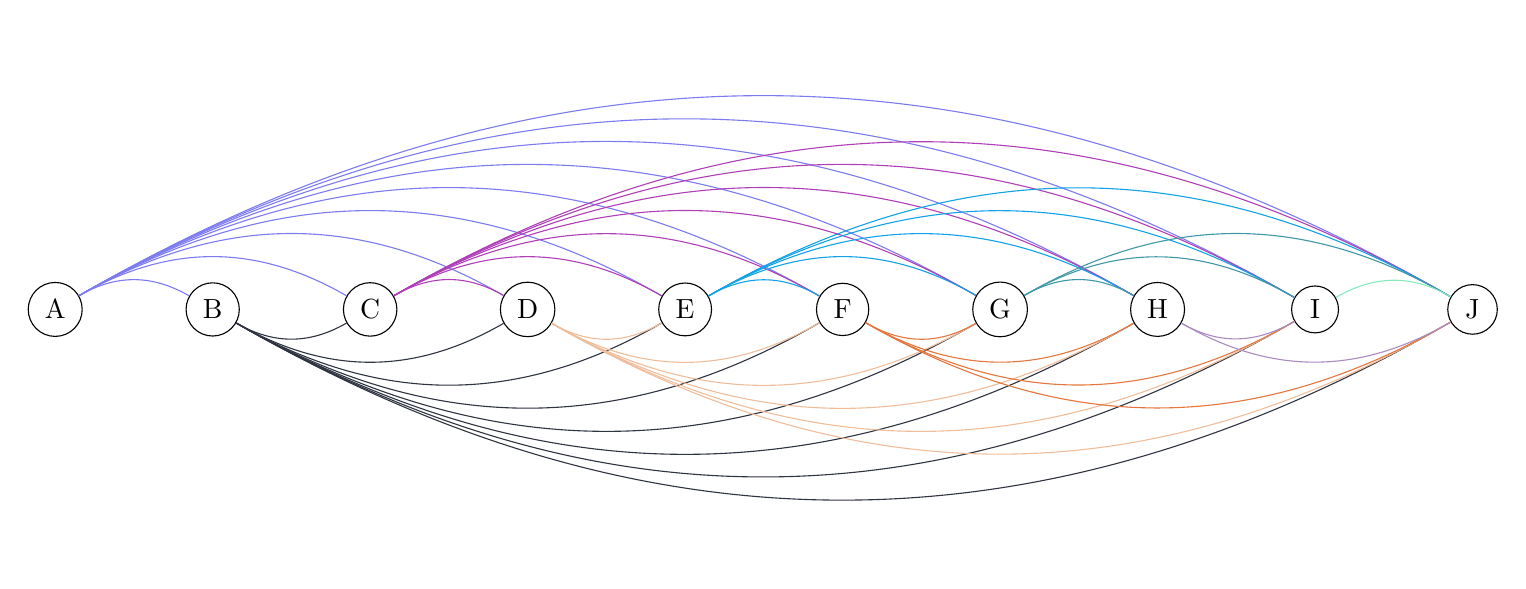
\begin{tikzpicture}
		\def\n{10}%Số ký tự theo bảng chữ cái
		\foreach \t in {1,...,\n}
		\path (2*\t,0) node[circle,draw] (\t) {\Letter{\t}};
		\pgfmathsetmacro{\nn}{int(\n-1)}
		\foreach \t in {1,...,\nn}{
			\pgfmathsetmacro{\to}{int(\t+1)}
			\pgfmathsetmacro{\out}{-30*(-1)^\t}
			\pgfmathsetmacro{\in}{-150*(-1)^\t}
			\pgfmathsetmacro{\R}{random(0,255)}
			\pgfmathsetmacro{\G}{random(0,255)}
			\pgfmathsetmacro{\B}{random(0,255)}
			\definecolor{randomcolor}{RGB}{\R,\G,\B}
			\foreach \tt in {\to,...,\n}
			\draw[randomcolor] (\t)to[out=\out,in=\in](\tt);
		}
	\end{tikzpicture}
\end{document}